\chapter{Sovellus}
\label{ch:sovellus}

Rippikoulujen sisältö pohjautuu rippikoulusuunnitelmaan
\parencite{evlSuuriIhmeRippikoulusuunnitelma2017}, joka määrittää pääraamit
muun muassa sille kaikelle, mitä rippikoulussa käsitellään. Yksi rippikoulun
tärkeistä osaalueista on isoset ja heidän osallistumisensa ohjelman
suunnitteluun ja järjestämiseen. Rippikoulusuunnitelmassa
\parencite{evlSuuriIhmeRippikoulusuunnitelma2017} mainitaankin:

\begin{quotation}
    \noindent Isoset ovat tärkeä osa rippikoulun kokonaisuutta ja myös
    rippikoulun tiimiä. Siksi seurakunnan isostoimintaa ja rippikoulujen
    kokonaisuutta kannattaa suunnitella yhdessä. Isosilla on keskeinen rooli
    rippikoululaisten samastumiskohteina ja ”isosisaruksina”. Rippikoululaiset
    oppivat usein isosilta enemmän kuin ohjaajilta.
\end{quotation}

Rippikoulusuunnitelmassa tuodaan esille se, että eri paikkakunnilla ja eri
seurakunnilla on erilaiset mahdollisuudet järjestää asioita. Tässä työssä
tilannetta katsellaan erityisesti Ruokolahden seurakunnan isosten näkökulmasta.

Ruokolahden seurakunnalla rippikoulu koostuu muun muassa kirkkokäynneistä,
nuortenilloista, etätehtävistä, opetuspäivistä ja lopulta varsinaisesta
leiristä. Vuoden aikana isoskoulutusta käyvät isoset sekä aiempina vuosina
isoskoulutuksen käyneet osallistuvat järjestämään ohjelmaa vuoden aikana
käytäviin nuorteniltoihin sekä ovat avustamassa jumalanpalveluksissa sekä
opetuspäivissä. Nämä ovat yksittäisiä pienempiä asioita, jotka saadaan
yleensä järjestettyä pienemmällä määrällä. Varsinaisella leirillä kuitenkin
tahti on toisenlainen. Parin tunnin ohjelman sijaan leiriläisille luodaan koko
leirin ajaksi ohjelma, joka sisältää toimintaa heräämisestä hiljaisuuteen asti.
Tähän tiiviiseen ohjelmaan pakataan kaikki asiat, joita rippikoululla käydään
läpi. Ohjelmarunko ja opetus on suunniteltu etukäteen, mutta elää tilanteen
mukaan ja harvemmin pysyy alkuperäisessä edes yhtä kokonaista päivää. Ohjelman
ollessa tiivis ja muutosten tullessa tilanteen tarvittaessa erittäin lyhyellä
varoitusajalla ja rippikoulutiimin koostuessa yleensä noin neljästä aikuisesta,
kymmenestä isosesta sekä vierailijoista, kuten kanttorista ja diakonissasta,
on tärkeää, että kaikki ovat ajantasalla milloin mitäkin tapahtuu. Ruokolahden
seurakunnalla tähän käytettiin pitkään ensisijaisesti ja ainuana keinona yhtä
ryhmäkeskustelua, johon kuuluivat kaikki, jotka olivat läsnä leirillä. Leirin
ollessa viikon mittainen, oli viimeisinä päivinä viestien määrä tuhansissa ja
mediaa, kuten kuvia ja pdf:iä, useita satoja. Tällöin sisällön etsintä muuttui
yhä hankalammaksi viikkoa loppuun mennessä ja tiedotetut muutokset olivat
pitkälti muistin varassa.

Tämän työn ohessa on luotu sovellus, joka pyrkii tuomaan helpostusta edellä
kuvattuun tilanteeseen ja keventämään erityisten isosten työkuormaa, mutta
samalla myös ohjaajien. Tulevaisuudeen on mietitty myös mahdollisuutta luoda
mahdollisuus leiriläisille sekä huoltajille nähdä leiriin liittyviä asioita
sovelluksesta. Toistaiseksi sovellus on kuitenkin vain ohjaajien ja isosten
käytössä.

Sovelluksesta löytyy kuvan \ref{fig:isosapp-leirit} mukaisesti kaikki leirit ja
leirien osallistujat, niin ohjaajat, isoset kuin leiriläisetkin. Leirillä
leiriläiset jaetaan leirillä isosryhmiin, jotka saadaan näkyviin leirin
päänykmään kuvassa \ref{fig:isosapp-ryhmat}.

\begin{figure}[h!]
    \centering
    \begin{minipage}[b]{.3\textwidth}
        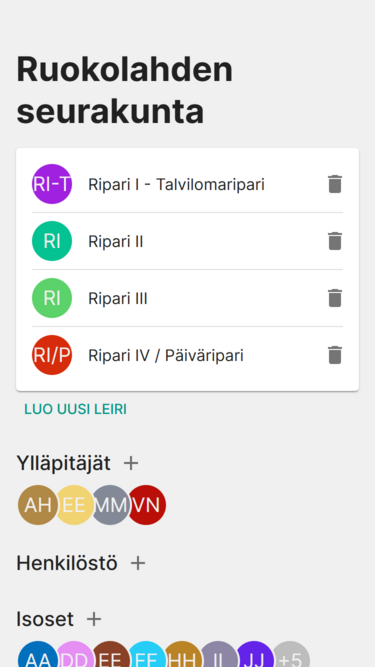
\includegraphics[width=\textwidth]{figures/isosapp-leirit.png}
        \caption{Seurakunnan näkymä, joka sisältää leirit, ohjaajat ja isoset}
        \label{fig:isosapp-leirit}
    \end{minipage}\qquad
    \begin{minipage}[b]{.3\textwidth}
        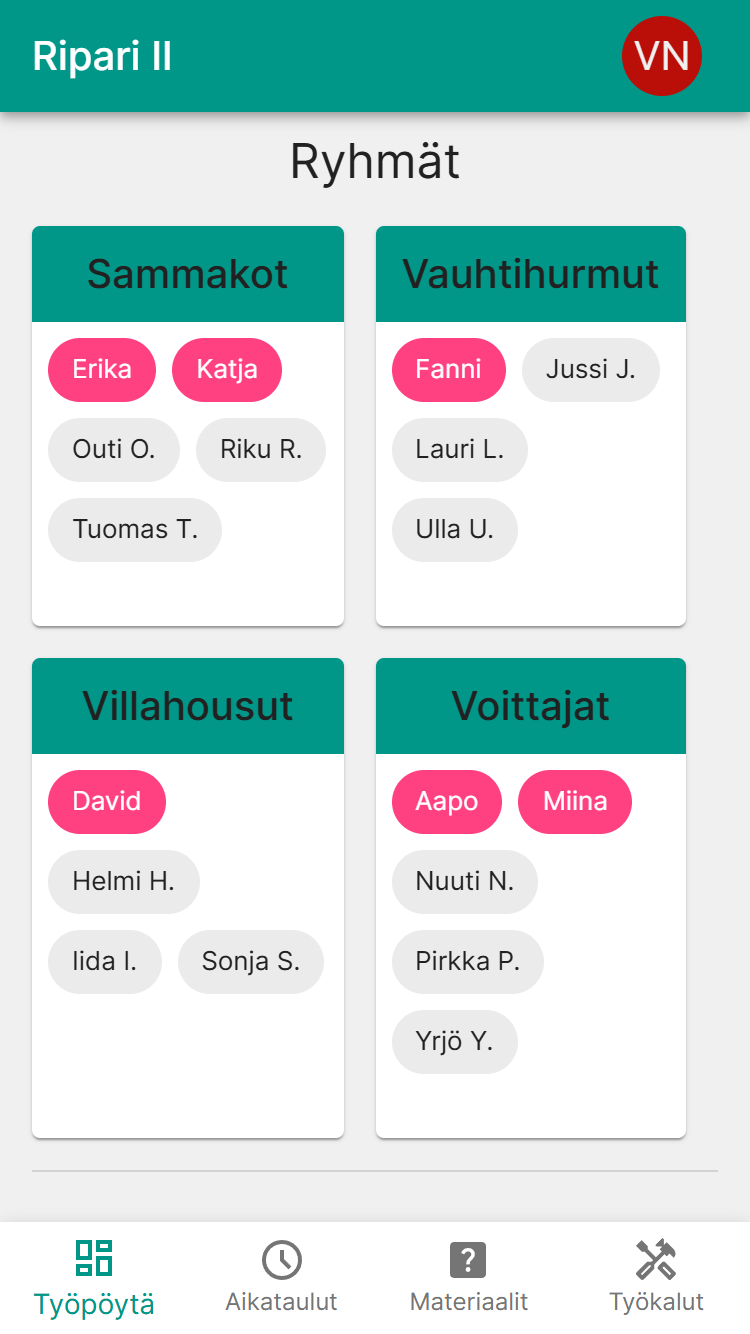
\includegraphics[width=\textwidth]{figures/isosapp-ryhmat.png}
        \caption{Leirin päänäkymän ryhmä-osio}
        \label{fig:isosapp-ryhmat}
    \end{minipage}
\end{figure}

Sovellus pohjautuu ensisijaisesti aikatauluun, jonka ympärille kaikki muu
leiriin liittyvä toiminnallisuus on rakennettu. Leirin päänäkymässä kuvassa
\ref{fig:isosapp-nakkilista} on jokaiselle näkyvissä henkilökohtainen
tehtävälista, joka näyttää seuraavan 24 tunnin sisällä olevat ohjelmat, joissa
on vetovastuuna. Samassa näkymässä on myös niin sanottu nakkilista, joka
sisältää päivittäin vaihtuvat roolit isosille. Varsinainen aikataulu löytyy
omasta näkymästä, joka on nähtävissä kuvassa \ref{fig:isosapp-aikataulu}.

\begin{figure}[h!]
    \centering
    \begin{minipage}[b]{.3\textwidth}
        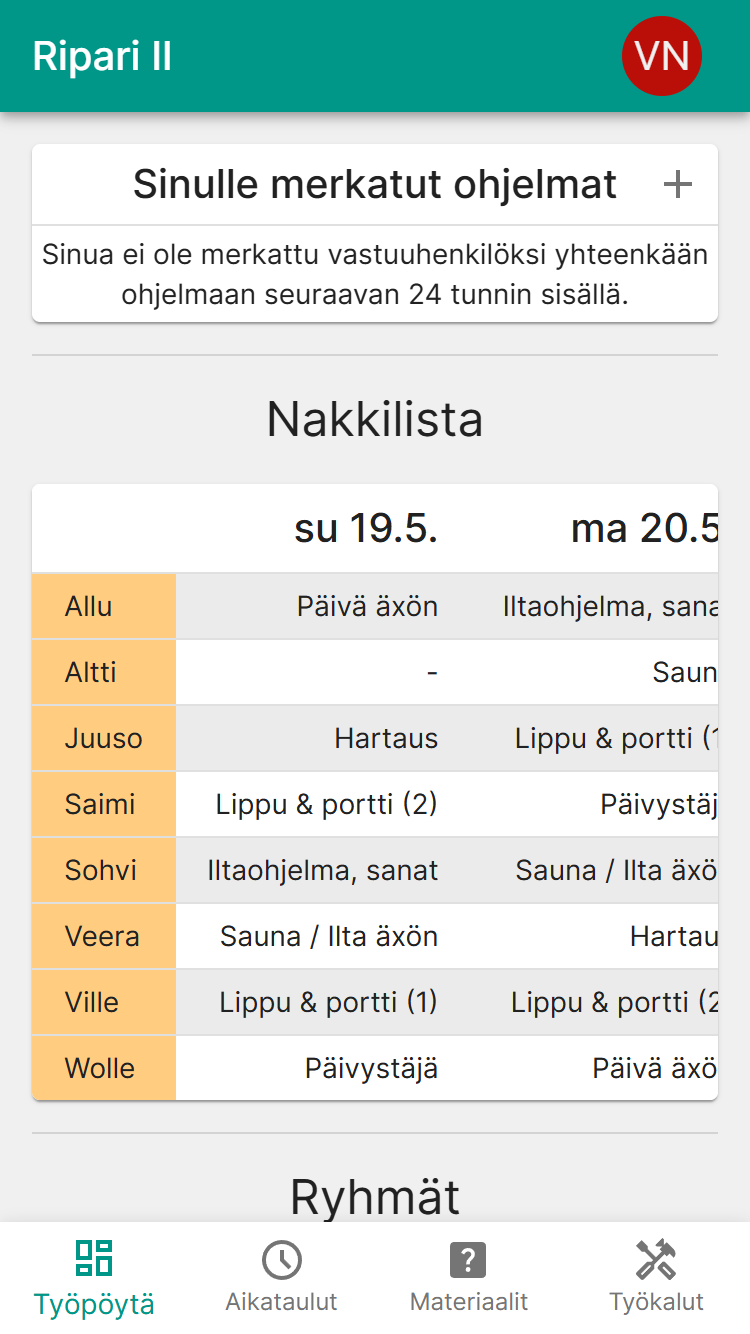
\includegraphics[width=\textwidth]{figures/isosapp-nakkilista.png}
        \caption{Leirin nakkilista ja henkilökohtainen tehtävälista}
        \label{fig:isosapp-nakkilista}
    \end{minipage}\qquad
    \begin{minipage}[b]{.3\textwidth}
        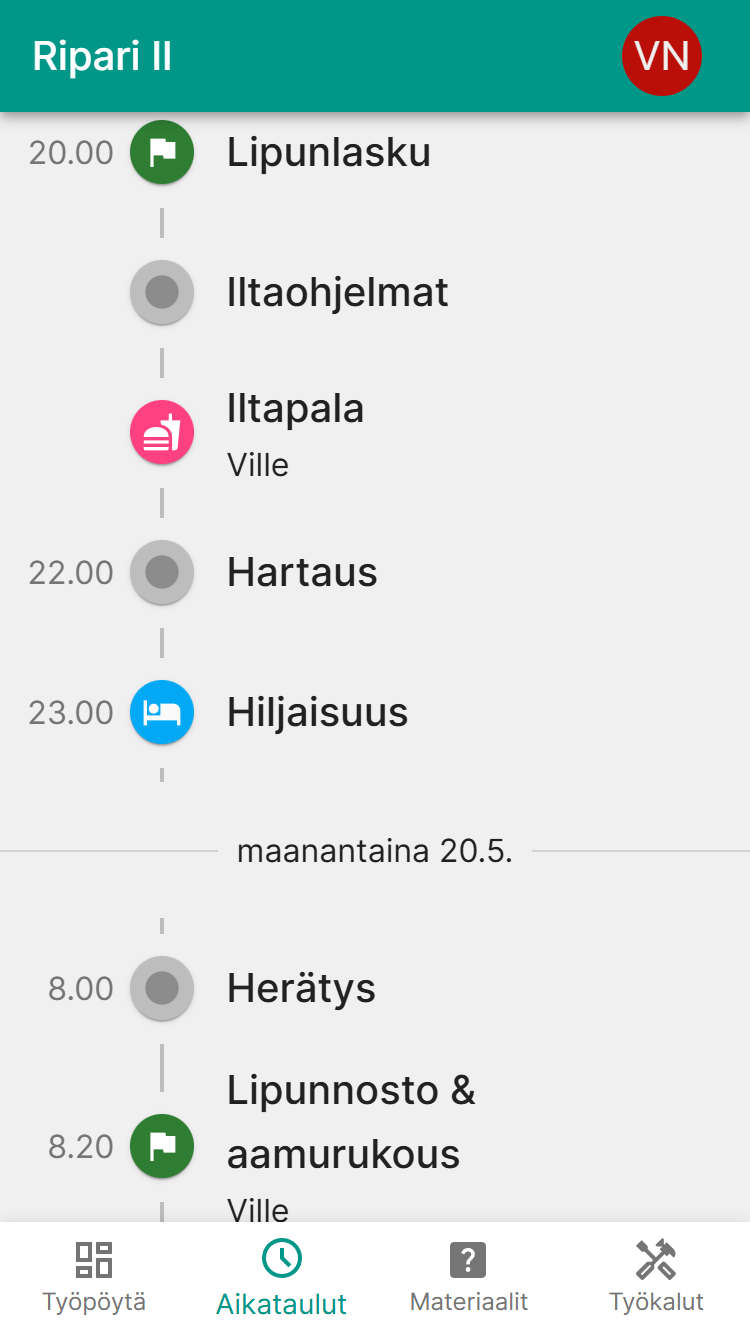
\includegraphics[width=\textwidth]{figures/isosapp-aikataulu.png}
        \caption{Leirin aikataulu ja ohjelmien vastuuhenkilöt}
        \label{fig:isosapp-aikataulu}
    \end{minipage}
\end{figure}

Näiden lisäksi ohjelman suunnittelua helpottamaan on luotu materiaalipankki,
josta löytyy kisoja, leikkejä ja sketsejä sekä listoja lauluista. Aikataulussa
oleviin ohjelmat on mahdollista linkittää suoraan materiaaliin, joten
ohjelmasta pääsee helposti näkemään mm. kilpailun säännöt, kuten kuvassa
\ref{fig:isosapp-materiaalit}. Materiaalin lisäksi ohjelman tekemisessä
tarvitaan välillä yksinkertaisia työkalua, kuten ryhmien arvontaa tai
telepromteria leikkimielisten uutisten lukemiseen. Näitä varten on luotu
kuvassa \ref{fig:isosapp-tyokalut} näkymä työkalu näkymä.

\begin{figure}[h!]
    \centering
    \begin{minipage}[b]{.3\textwidth}
        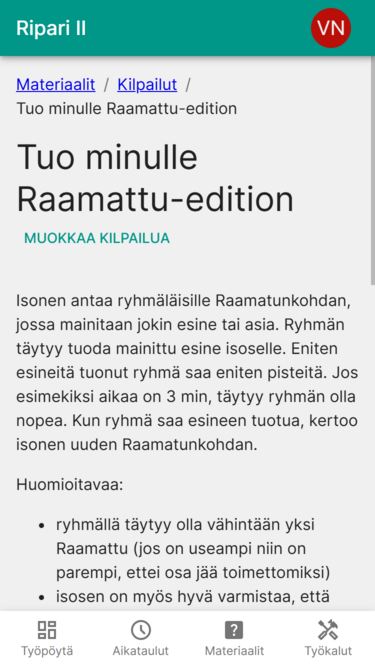
\includegraphics[width=\textwidth]{figures/isosapp-materiaalit.png}
        \caption{Esimerkki materiaaleihin lisätystä kilpailusta}
        \label{fig:isosapp-materiaalit}
    \end{minipage}\qquad
    \begin{minipage}[b]{.3\textwidth}
        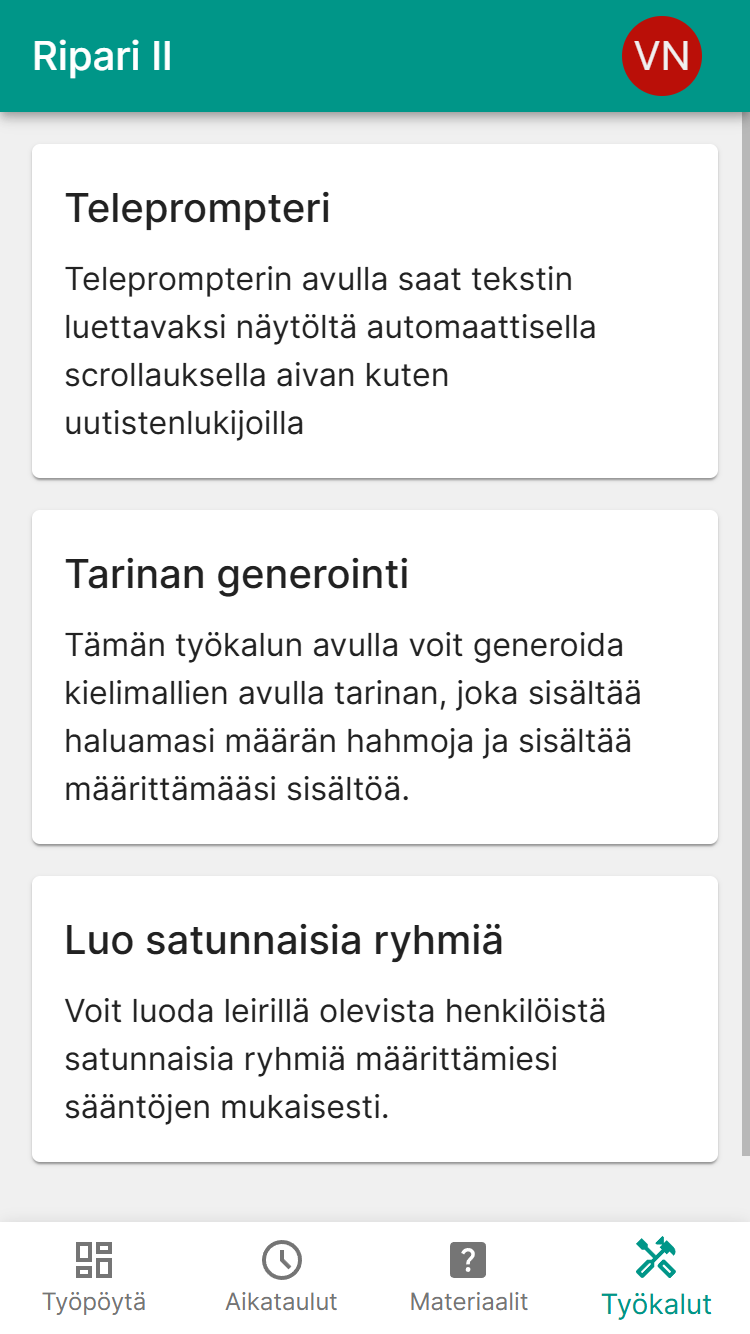
\includegraphics[width=\textwidth]{figures/isosapp-tyokalut.png}
        \caption{Sovelluksen työkalu-näkymä}
        \label{fig:isosapp-tyokalut}
    \end{minipage}
\end{figure}

\clearpage
\section{Kielimallien integrointi osaksi sovellusta}

\begin{wrapfigure}{r}{0.45\textwidth}
    \centering
    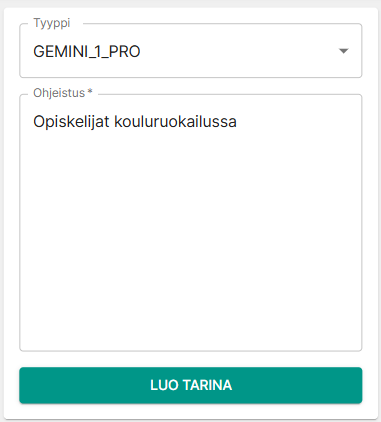
\includegraphics[width=0.45\textwidth]{figures/isosapp-tyokalut-tarinan-generointi-1.png}
    \caption{Tarinan luontinäkymä}
    \label{fig:isosapp-tyokalut-tarinan-generointi-1}

    \qquad

    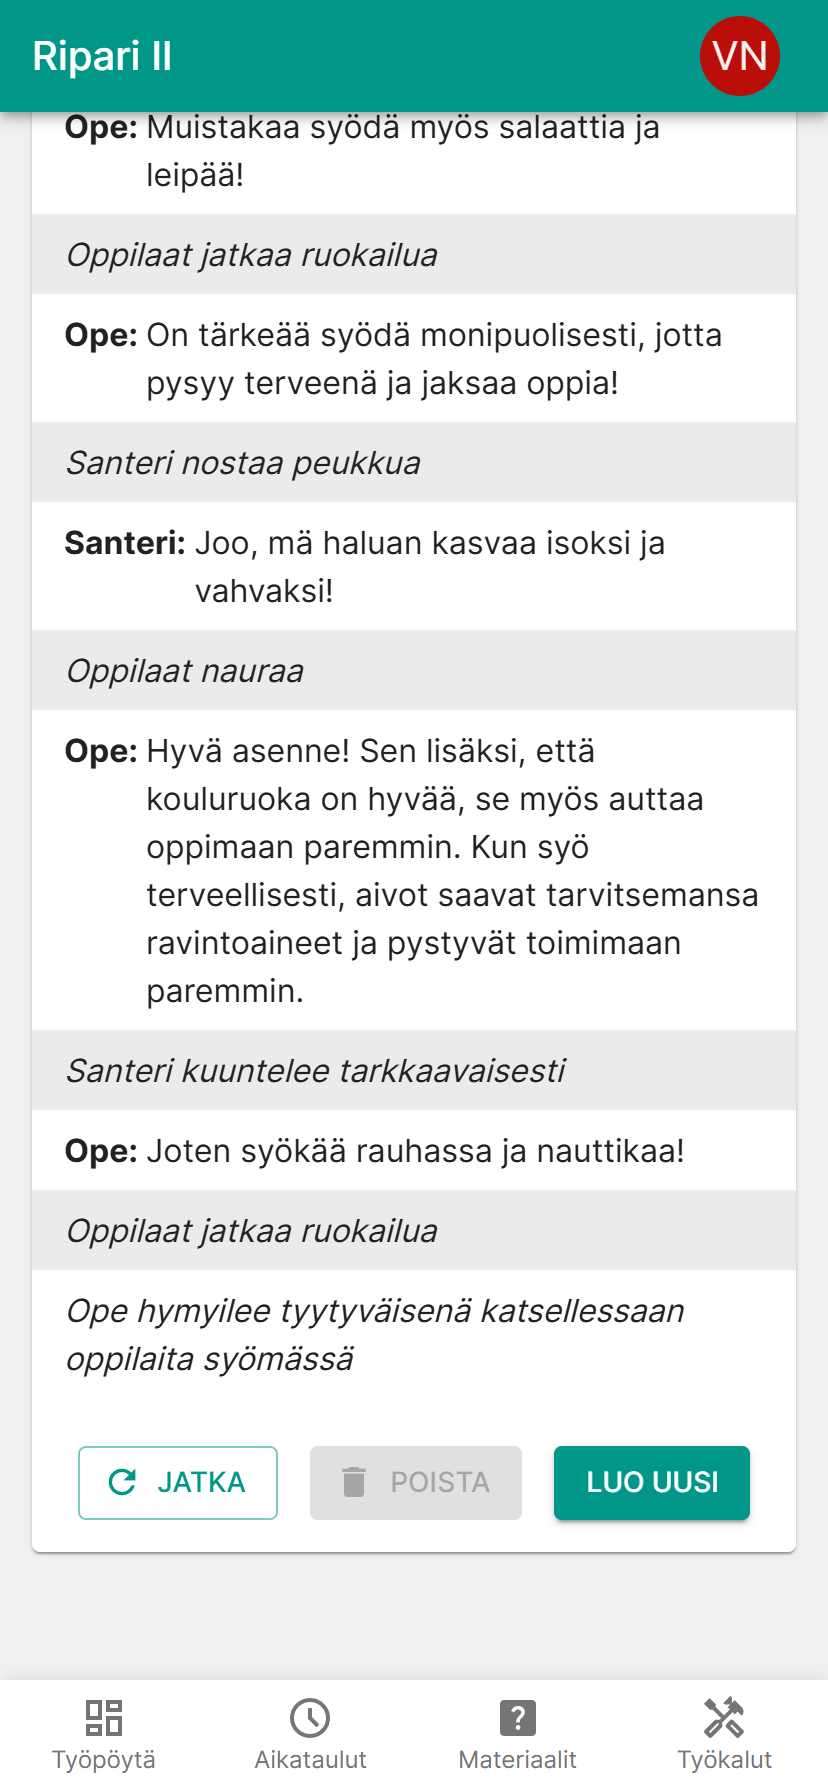
\includegraphics[width=0.45\textwidth]{figures/isosapp-tyokalut-tarinan-generointi-2.png}
    \caption{Sovelluksen työkalu-näkymä}
    \label{fig:isosapp-tyokalut-tarinan-generointi-2}
\end{wrapfigure}

Kielimallit ovat hyviä tuottamaan paljon sisältöä ja nopeasti. On tilanteita,
joissa tällaisesta on hyötyä, vaikka sisältöä ei olisikaan laadullisesti
parasta mahdollista. Yhtenä esimerkkinä tästä on työkalu, jolla saa generoitua
tarinaa. Tätä tarinaa voidaan käyttää pohjana muun muassa sketsien luomisessa.

Sovellukseen on toteutettu kielimalleja hyödyntävä työkalu, jolle saa valittua
käytettävän kielimallin ja annettua ohjeistuksen, mitä tarinan tulisi sisältää,
kuvan \ref{fig:isosapp-tyokalut-tarinan-generointi-1} mukaisesti.
Käyttöliittymä osaa näyttää tarinan vuorosanat sekä toiminnot, kuten kuvassa
\ref{fig:isosapp-tyokalut-tarinan-generointi-2} nähdään. Käyttöliittymä tukee
myös tarinan jatkamista mikäli vain valittulle kielimmallille on toteutettu
kyseinen toiminnallisuus backendin puolelle.

Työkalun lähtökohtana ollut päästä testaamaan useampaa eri kielimallia, joten
toteutuksesta on pyritty tekemään mahdollisimman joustava useammalla eri
kielimallille. Jokaisen kielimallin toteutuksen tulee toteuttaa
\ref{lst:StoryLineService.java} interfacen kaikki metodit, jotta kielimallia
saadaan käytettyä olemassa olevan käyttöliittymän kanssa. Metodit heittää
poikkeuksen, mikäli suoritus ei onnistunut, jolloin käyttöliittymä näyttää
virheen ja mahdollistaa uudelleen yrittämisen.

\clearpage
\begin{lstlisting}[
    basicstyle=\small,
    caption={StoryLineService interface, jonka toteuttamalla kielimallit saadaan },
    label={lst:StoryLineService.java},
    language=java,
]
public interface StoryLineService {

    List<StoryLine> createStoryLines(Story story);
    List<StoryLine> continueStoryLines(Story story);
    void cleanUp(Story story);
}
\end{lstlisting}

\subsection{Gemini toteutus}

Aiemmin \ref{lst:GeminiService.java} kohdassa esiteltyyn GeminiService saadaan
toteuttamaan StorylineService-interface liitteen \ref{ch:gemini-service}
mukaisesti, jonka jälkeen kielimallilla saadaan tuotettua esimerkiksi kuvassa
\ref{fig:isosapp-tyokalut-tarinan-generointi-2} näkyvä tarina.

TODO: kattavampi selitys toteutuksesta

\subsection{PaLM2 toteutus}

Vastaavasti \ref{lst:PaLM2Service.java} kohdassa esitelty PaLM2Service saadaan
toteuttamaan StorylineService-interface liitteen \ref{ch:palm2-service}
mukaisesti. PaLM 2:lle ei ole tarjolla vastaavaa ChatSessionia, kuin Geminille,
joten on sille toteutettu vain tarinan luonti, muttei mahdollisuutta jatkaa
tarinaa.

TODO: kattavampi selitys toteutuksesta

\subsection{xAI:n toteutus}

XAI:n rajapinnan dokumentaatiossa on määritelty 'response\_format'-kenttä, mutta
kyseiselle kentälle ei ole määritelty tyyppiä \parencite{xAIDocsEndpoints}.
Mahdollinen formaatti kyseiselle kentälle löydetään Githubissa olevasta
issuesta \parencite{githubBerriAIlitellmIssues6610}, jossa ongelmana on se,
ettei vastauksen formatointi ole tuettu sillä hetkellä. Testaamalla samalla
formaatilla saamme itsekkin vastauksena kohdassa \ref{lst:xai-bad-request.json}
näkyvän virheviestin ettei ainakaan kyseinen formatointi ole käytössä.

\begin{lstlisting}[
    basicstyle=\small,
    caption={XAI rajapinnan palauttama vastaus, kun yritetään määrittää 'response\_format'-kenttä},
    label={lst:xai-bad-request.json},
]
{
    "code":"Client specified an invalid argument",
    "error":"The model does not support formatted output but some
      have been specified in the request."
}
\end{lstlisting}

Vaikkei rajapinta suoraan vaikuta tukevan vastauksen muotoilua, voidaan ohjeet
muotoiluun antaa kirjallisesti. Alustamalla keskustelu system-roolilta
tulevalla viestillä:

\begin{quotation}
    \noindent Olet käsikirjoittaja. Luot tarinan käyttäjän antaman syötteen
    perusteella.

    \noindent Vastauksesi tulee olla JSON-muodossa oleva lista, joka koostuu
    olioista, joilla on kolme attribuuttia: type, target ja content. Type voi
    olla joko `ACTION` tai `TALK` riippuen siitä, onko kyseessä jotakin mitä
    tapahtuu vai jotain mitä joku sanoo. Target kuvastaa sitä kuka tekee tai
    kuka sanoo. Content kuvastaa sitä mitä tapahtuu tai sanotaan.
\end{quotation}

saadaan vastaukset halutussa JSON-muodossa, jonka myötä saadaan viesti
parsittua StoryLineService-interfacen metodien vastauksien haluamaan
muotoon antamalla vastaus suoraan JSON-parserille kohdan
\ref{lst:XAIService.java::parseResponse} mukaisesti.

\begin{lstlisting}[
    basicstyle=\small,
    caption={XAI rajapinnan palauttaman vastauksen parsiminen haluttuun muotoon},
    label={lst:XAIService.java::parseResponse},
    language=java,
]
private List<StoryLine> parseResponse(Message message)
    throws IOException
{
    // Luetaan viestin sisältö ja poistetaan ylimääräinen muotoilu
    String json = message.content()
        .replaceFirst("```json\n", "")
        .replaceFirst("```", "");

    // Luetaan tekstimuodossa oleva json listaksi StoryLine-olioita
    return objectMapper.readValue(json, new TypeReference<>() {});
}
\end{lstlisting}

Käytettävä rajapinta päätepiste pohjautuu alunperinkin siihen, että sinne
lähetetään lista viesteistä. Tätä hyödyntämällä pystymme toteuttamaan
toiminnallisuuden tarinan jatkamiseen. Pitämällä kirjaa aiemmista viesteistä
voimme tarinan jatkamisessa yksinkertaisesti hakea vanhat viestit ja pyytää
jatkamaan tarinaa kuten kohdassa \ref{lst:XAIService.java::continueStoryLines}
olevassa toteutuksessa on tehty.

\begin{lstlisting}[
    basicstyle=\small,
    caption={XAI rajapinnan palauttaman vastauksen parsiminen haluttuun muotoon},
    label={lst:XAIService.java::continueStoryLines},
    language=java,
]
public List<StoryLine> continueStoryLines(Story story) {
    // Haetaan keskustelun vanhat viestit
    List<Message> messages = chats.get(story.getId());

    // Tarkistetaan ettei tarina kasva liian pitkäksi
    if (story.getLines().size() > 50 || messages.size() > 10)
        throw new BadRequestException("Tarina on liian pitkä!");

    // Lisätään käyttäjän pyyntö jatkaa tarinaa
    messages.add(new Message("user", "Jatka tarinaa"));

    // tehdään pyyntö
    // parsitaan vastaus
    // palautetaan uudet rivit
}
\end{lstlisting}
